\documentclass{standalone}
\usepackage{tikz}
\usepackage{amsmath}
\usepackage{amssymb}
\usetikzlibrary{arrows.meta, positioning, calc, backgrounds}

\begin{document}
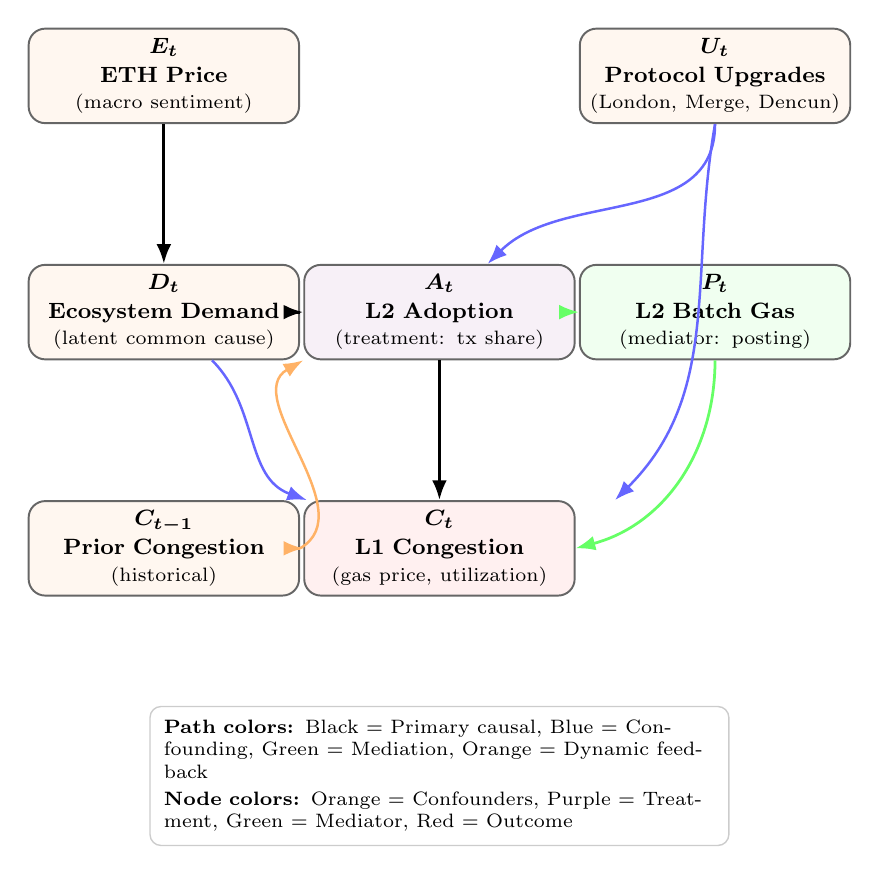
\begin{tikzpicture}[
  node distance = 3cm and 4cm,
  every node/.style = {
    rounded corners=6pt,
    draw=black!60,
    align=center,
    font=\footnotesize,
    fill=blue!5,
    minimum height=1.2cm,
    text width=3.2cm,
    line width=0.7pt
  },
  arrow/.style = {-{Latex[length=2.5mm]}, thick},
  confounder/.style = {fill=orange!6},
  mediator/.style = {fill=green!6},
  treatment/.style = {fill=violet!6},
  outcome/.style = {fill=red!6}
]

% Layer 1: Macro drivers (top row)
\node[confounder] (E) at (0,0) {$\boldsymbol{E_t}$\\[1pt]\textbf{ETH Price}\\{\scriptsize (macro sentiment)}};

\node[confounder] (U) at (7,0) {$\boldsymbol{U_t}$\\[1pt]\textbf{Protocol Upgrades}\\{\scriptsize (London, Merge, Dencun)}};

% Layer 2: Ecosystem demand (left side)
\node[confounder] (D) at (0,-3) {$\boldsymbol{D_t}$\\[1pt]\textbf{Ecosystem Demand}\\{\scriptsize (latent common cause)}};

% Layer 3: Treatment (center)
\node[treatment] (A) at (3.5,-3) {$\boldsymbol{A_t}$\\[1pt]\textbf{L2 Adoption}\\{\scriptsize (treatment: tx share)}};

% Layer 4: Mediator (right side)
\node[mediator] (P) at (7,-3) {$\boldsymbol{P_t}$\\[1pt]\textbf{L2 Batch Gas}\\{\scriptsize (mediator: posting)}};

% Layer 5: Dynamic feedback (bottom left)
\node[confounder] (Cprev) at (0,-6) {$\boldsymbol{C_{t-1}}$\\[1pt]\textbf{Prior Congestion}\\{\scriptsize (historical)}};

% Layer 6: Outcome (bottom center)
\node[outcome] (C) at (3.5,-6) {$\boldsymbol{C_t}$\\[1pt]\textbf{L1 Congestion}\\{\scriptsize (gas price, utilization)}};

% === ARROWS (without overlapping labels) ===

% Primary causal paths (thick black)
\draw[arrow, line width=1.1pt] (E) -- (D);
\draw[arrow, line width=1.1pt] (D) -- (A);
\draw[arrow, line width=1.1pt] (A) -- (C);

% Confounding paths (blue)
\draw[arrow, blue!60, line width=0.9pt] (D) to[out=-45, in=160] (C);
\draw[arrow, blue!60, line width=0.9pt] (U) to[out=-90, in=45] (A);
\draw[arrow, blue!60, line width=0.9pt] (U.south) to[out=-100, in=45] ([xshift=0.5cm]C.north east);

% Mediation paths (green)
\draw[arrow, green!60, line width=1pt] (A) -- (P);
\draw[arrow, green!60, line width=1pt] (P) to[out=-90, in=15] (C.east);

% Dynamic feedback (orange)
\draw[arrow, orange!60, line width=0.9pt] (Cprev.east) to[out=30, in=-150] (A.south west);
\draw[arrow, orange!60, line width=0.9pt] (Cprev) -- (C);

% === LEGEND ===
% Place legend below the main diagram
\node[draw=gray!40, fill=white!98, rounded corners=4pt,
      font=\scriptsize, align=left, text width=7cm,
      anchor=north, inner sep=5pt, line width=0.5pt]
      at (3.5,-8) {
    \textbf{Path colors:} Black = Primary causal,
    Blue = Confounding,
    Green = Mediation,
    Orange = Dynamic feedback\\[2pt]
    \textbf{Node colors:} Orange = Confounders,
    Purple = Treatment,
    Green = Mediator,
    Red = Outcome
};

\end{tikzpicture}
\end{document}